Jako první určíme rozměry tranzistoru zrcadla.
Volím délku kanálu \(L = 2 [\mu m]\) jako kompromis mezi velikostí a parametrem \(\lambda\) která pro \(L = 2 \mu m\) nabívá hodnoty \(\lambda = 0.0787698 [V^{-1}]\).
Dále musíme zvolit napětí \(U_{OV}\) které volím s ohledem na rozsah napájecího napětí \(U_{OV} = 0.2 [V]\)
Z toho následně můžeme určit šířku kanálu \(W\), tranzistorů \(M2\) a \(M3\) jako:

\begin{center}
    \large
    \(
        W_{M2} = W_{M3} = L \cdot \frac{2 \cdot I_1}{KP \cdot U_{OV}^2} = 2\mu \cdot \frac{2 \cdot 10\mu}{50\mu 0.2^2} = 20 [\mu m]
    \)
\end{center}

Z Toho snadno určíme \(W_{M4}\) a \(W_{5}\) jako:

\begin{center}
    \large
    \(
        W_{M4} = W_{M5} = W_{M2} \cdot \frac{I_2}{I_1} = 20\mu \cdot \frac{20\mu}{10\mu} = 40 [\mu m]
    \)
\end{center}

Výstupní odpor pak můžeme určit jako:

\begin{center}
    \large
    \(
        r_{out} = g_{m-M4} \cdot r_{DS-M4} \cdot r_{DS-M5} = g_{m-M4} \cdot \frac{1}{\lambda_{M4}\cdot I_{M4}} \cdot \frac{1}{\lambda_{M5}\cdot I_{M5}} = 73.2\mu \cdot \frac{1}{0.0787698 \cdot 20\mu} \cdot \frac{1}{0.0787698 \cdot 20\mu} = 29.5 [M \Omega]
    \)
\end{center}

A výstupní rozsah jako:

\begin{center}
    \large
    \(
        U_{out} = U_{CC} - (U_{OV-M5} + U_{OV-M4} + U_{TH-M4}) = 1.8 - (0.2+0.2+0.427) = 0.97 [V]
    \)
\end{center}

\vspace{10mm}
\begin{figure}[h!]
    \centering
    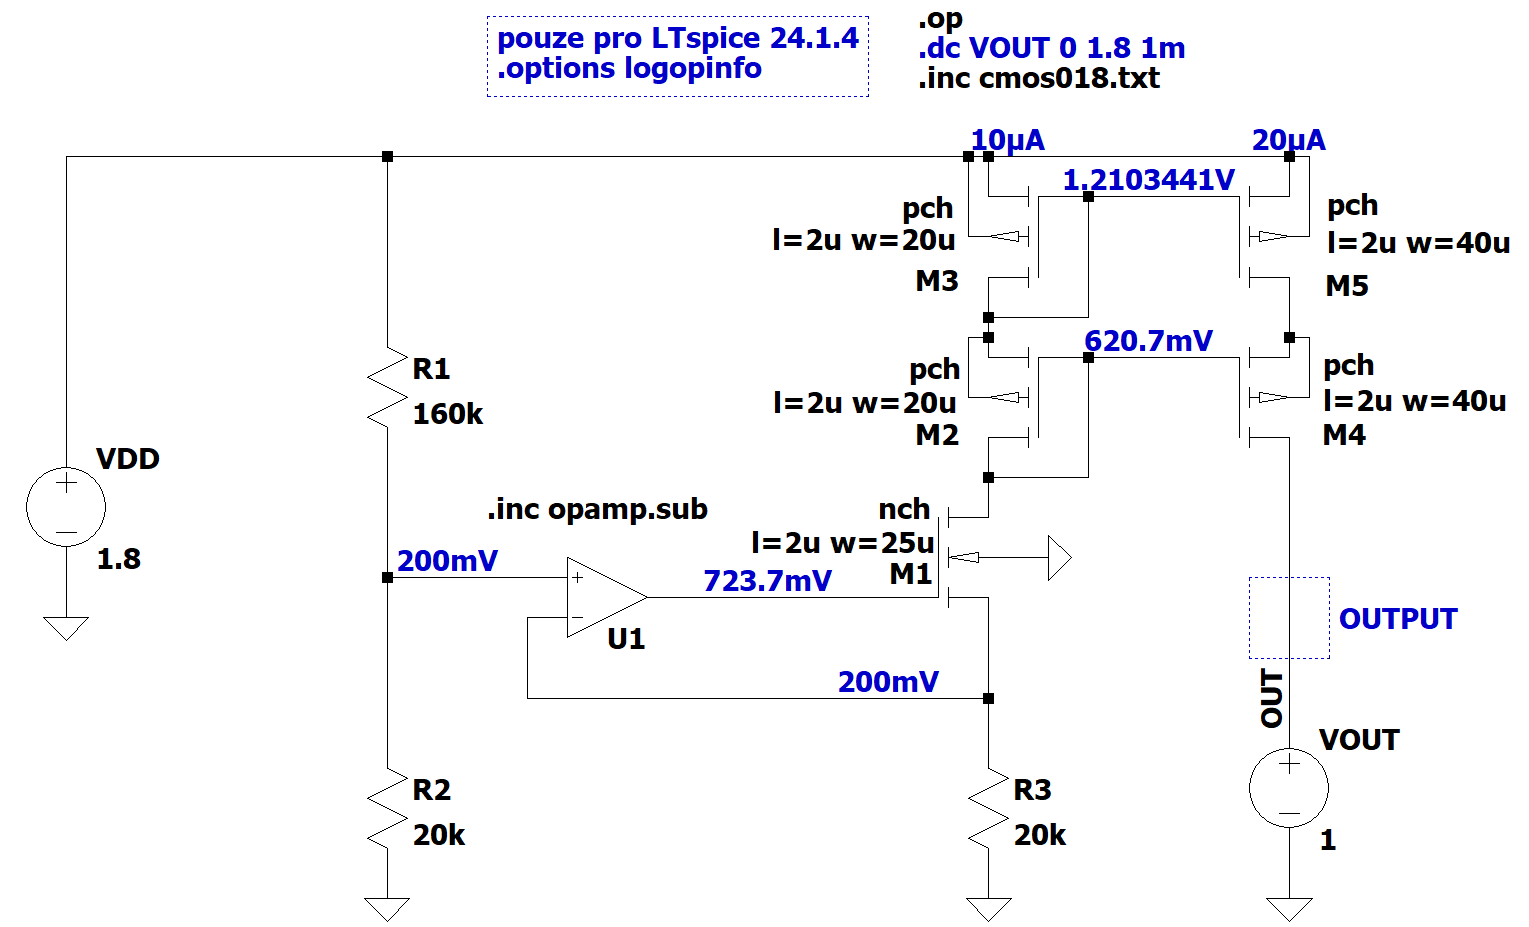
\includegraphics[width=0.9\textwidth]{text/img/KPZ-op-sch.png}
    \caption{\label{fig:KPZ-op-sch} zobrazení napětí a proudu ve schématu}
\end{figure}

\begin{figure}[h!]
    \centering
    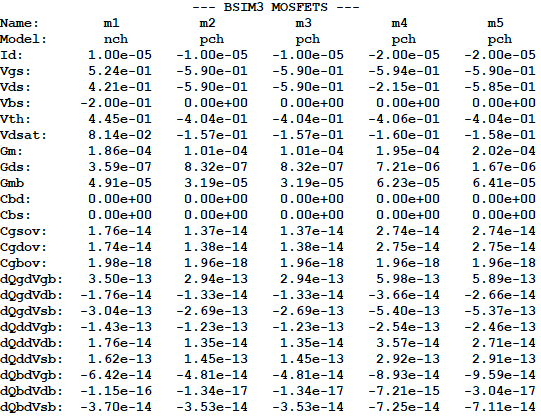
\includegraphics[width=0.9\textwidth]{text/img/KPZ-op-OL.png}
    \caption{\label{fig:KPZ-op-OL} Pracovní body jednotlivých tranzistorů}
\end{figure}

\newpage

\begin{figure}[h!]
    \centering
    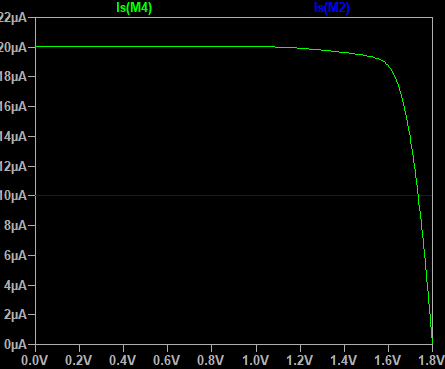
\includegraphics[width=0.9\textwidth]{text/img/KPZ-dc-graf.png}
    \caption{\label{fig:KPZ-dc-graf} Simulovaná závislost výstupího proudu na výstupním napětí}
\end{figure}

\begin{figure}[h!]
    \centering
    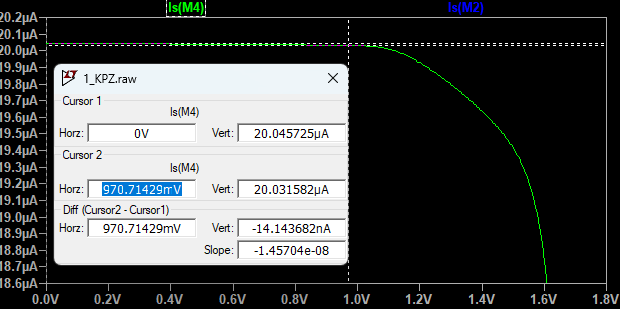
\includegraphics[width=0.9\textwidth]{text/img/KPZ-dc-graf-detail.png}
    \caption{\label{fig:KPZ-dc-graf-detail} Simulovaná závislost výstupího proudu na výstupním napětí v detailu}
\end{figure}

Z grafu \ref{fig:KPZ-dc-graf-detail} můžeme odečíst pokles hodnoty proudu na obou stranách pracovního rozsahu a i přímo jejich změny \(\Delta I = 14.14 [nA]\) při změně napětí \(\Delta U = 970.7 [mV]\).
Výstupní odpor tak můžeme určit jako:

\begin{center}
    \large
    \(
        r_{out} = \frac{\Delta U}{\Delta I} = \frac{970.7m}{14.14n} = 68.2 [M\Omega] 
    \)
\end{center}

Tato hodnota je cca poloviční ve srovnání s výpočtem, původně jsem předpokládal že mám špatné hodnoty \(\lambda\) ale ani po kontrole a opravě jsem nedošel k výsledkům podobným simulaci.

Výstupní rozsah odpovídá naproti tomu výpočtu velmi přesně a na průběhu je i vidět dvě místa kde dochází ke změnám výstupního odporu.
Nejdřív menší změna hned za koncem rozsahu když začne \(M4\) přecházet do lineárního režimu a následně vetší změna když začne vstupovat do lineárního režimu i \(M5\).